\documentclass[a4paper,11pt]{article}
%\usepackage{array}
%\usepackage{theorem}
\usepackage{graphicx}
\usepackage{fancyhdr}
\usepackage[toc,page]{appendix}
%\usepackage{times,mathptm}
%\usepackage[pdftex]{graphicx}
%\usepackage{color}
%\usepackage{caption}
%\usepackage{graphpap}
%\usepackage{rotating}
%\usepackage{epsfig}
%\usepackage{epsfig,psfrag}

%\setlength{\textwidth}{6.0in}
%\setlength{\textheight}{8.0in}
%\setlength{\topmargin}{0.in}
%\setlength{\headheight}{0.8in}
%\setlength{\headsep}{0.in}
%\setlength{\parindent}{0.25in}
%\setlength{\oddsidemargin}{0.2in}
%\setlength{\evensidemargin}{0.2in}

\newcommand{\ve}[1]{\mbox{\boldmath $ #1$}}
%opening
\title{TDStool: Notes on Numerical Methods}
\author{Andrea Bertoni, Thomas Serafini}



\begin{document}

%\setlength{\leftmargini}{\parindent} % Controls the indenting of the "bullets" in a list
%\pagestyle{empty}
%\pagenumbering{alph}
%\begin{minipage}[t][7.5in][s]{6.25in}
\begin{titlepage}

\flushright{
\Huge
TDS{\hspace{1mm}}tool}

\flushright{
\LARGE
\mbox{Time Dependent Schr{\"o}dinger equation simulation tool}}

\vspace{40mm}
\flushright{
\huge
\bf Notes on Numerical Methods}

\vspace{20mm}
\flushright{
\Large
Andrea Bertoni \\
\vspace{2mm}
Thomas Serafini}

\vspace{60mm}
\flushright{
\large
\today \\
Version 0.2 \\
TDStool Version 0.2}

\vspace{10mm}
\flushright{
\Large
S3 National Research Center, CNR-INFM \\ Modena, Italy}

\normalsize
%\vfill
% \flushright{\includegraphics[width=2.in]{FIGURES/nistident_flright_vec}}

\newpage
\pagestyle{empty}
\mbox{}
\end{titlepage}
%\end{minipage}
%\maketitle
%\begin{abstract}
%\end{abstract}

\section*{Preface}
The software TDStool is a numerical solver for the Time Dependent (linear)
Schr\"odinger equation and (nonlinear) Gross-Pitaevskii equation.
This document provides the theoretical basis for TDStool.
It describes the discretization methods and the main numerical
algorithms used in the code. It aims to be a technical reference guide
and a means to reach an in-depth understanding of the source code.
In fact, it should be the starting point for whoever is willing to
modify the code (released as an open-source project) and hopefully contribute
to the project.
Since the discussion in this note has been kept at a tutorial level, 
it can represent a nimble introduction to some of the numerical techniques
used in the code. However, we urge newcomers to read the references
suggested in the text.

\section*{Disclaimer}
We make no warranty to users of TDStool and accept no responsability for
its use and for any conclusion drawn from its results.  Although we endeavor
to provide an easy-to-use software with an intuitive interface, TDStool is
primarily intended for use by those competent in the field of quantum mechnaics
and numerical analysis.

\section*{Copyright}
At this early stage, the software TDStool and the related documentation
(including the present note) is copyrighted by the authors and their
employer.  The TDStool code is released as open-source and is free for
personal use.  We plan to release a later version of the siftware with a public
license.


\section*{About the Authors}
%(up-to-date as of \today)

{\bf Andrea Bertoni} is

{\bf Thomas Serafini} is

\section*{Acknowledgments}
TDStool has been developed within the \emph{TDStool} INFM Seed project 2008.
We are pleased to thank Guido Goldoni (Universit\`a di Modena e Reggio Emilia)
and Massimo Rudan (Universit\`a di Bologna) for most helpful discussions and
suggestions.

\newpage

\tableofcontents

\newpage

\pagestyle{fancy}
\fancyhead[RO,RE]{TDStool: Notes on Numerical Methods}
\fancyhead[LO,LE]{ver. 0.2}


\section{Introduction}
The single-particle dynamics of a nonrelativistic quantum system follows
the so-called time-dependent Schr\"odinger equation (TDSE) that relates the time derivative
of the system state with the system Hamiltonian ${\cal H}$ and the state itself.
In the real-space representation, for a spinless particle the TDSE is the partial differential equation 
\begin{equation} \label{tdse1}
i\hbar\frac{\partial}{\partial t}\psi({\bf r},t)= {\cal H} \psi({\bf r},t),
\end{equation}
where ${\bf r}$ is the position, $t$ the time coordinate, $\psi({\bf r},t)$ a complex-valued
function representing the quantum state, with $|\psi({\bf r},t)|^2$ the probability density in
${\bf r}$ and $t$.  The Hamiltonian ${\cal H}$ in the above
equation is a differential operator written in the real-space representation.

The aim of TDStool is to solve numerically Eq.~(\ref{tdse1}) once the initial condition
$\psi({\bf r},t=0)$ and a proper bondary condition on the computational domain are given.

We will first deal with a single particle moving in a static scalar (e.g. electric) potential,
then we will generalize the discussion to include time-dependent fields. 
The effect of a time-dependent
uniform magnetic field will be added in a future version of these notes.

For the sake of brevity, we will only consider 2D systems and domains, i.e. with ${\bf r}=(x,y)$.
Formulas for different dimensionality will be explicitely reported only if the generalization
is not straightforward. Where manifest, the spatial or time coordinates of the wave function will
be implied.


\section{Schr\"{o}dinger equation with a scalar potential}

We consider a single particle subject to a potential $U(x,y,t)$, eventually dependent
on the time $t$.
We want to solve the TDSE Eq.~(\ref{tdse1}) on a rectangular domain
\begin{equation}
D = (x,y) \mid x\in[0,X], y\in[0,Y]
\end{equation}
with given $X$ and $Y$.
We assume Dirichlet conditons on the domain boundaries
\begin{equation}
\partial(D) = (0,y) \cup (X,y) \cup (x,0) \cup (x,Y) \mid x\in[0,X], y\in[0,Y]
\end{equation}
i.e. the values of the wave function $\psi(x,y,t)$ in the points $(x,y)\in\partial(D)$ are given.

The Hamiltonian of the system reads $ {\cal H} = - \frac{\hbar^2}{2m}\nabla^2 + U(x,y,t) $,
where $m$ is the mass of the particle.
Equation~(\ref{tdse1}) becomes the standard real-space TDSE for a single particle in a scalar
potential:
\begin{equation} \label{tdsestatic}
i\hbar \frac{\partial \psi}{\partial t} = - \frac{\hbar^2}{2m}\nabla^2 \psi(x,y,t)
+ U(x,y,t)\psi(x,y,t) .
\end{equation}


\section{Box Integration Method}

In order to discretize the spatial coordinates of the TDSE we employ
the Box Integration Method, also known as Finite Volume Method.
We start by semidiscretizing the Schr\"{o}dinger equation in the space.
We work on the above special case where the domain $D$ is a box and we take
an orthogonal and separable discretization grid.
We are going to consider a 2D grid, but the discretization can easily be
extended to a higher dimensional domain.
Furthermore, for brevity we rewrite Eq.~(\ref{tdsestatic}) as
\begin{equation} \label{tdsenoconst}
\frac{\partial \psi}{\partial t} = -\beta \nabla G + v \, \psi \, ,
\end{equation}
where we have used the definitions
\begin{eqnarray}
\beta &=& i \frac{\hbar}{2m} , \\
v &=& \frac{1}{i \hbar} U , \\
G &=& \nabla \psi \, .
\end{eqnarray}

Let $ x_0 < x_1 < \cdots < x_{N+1} $ and $ y_0 < y_1 < \cdots < y_{M+1} $ be the coordinates of an
orthogonal grid, with $x_0=0$, $x_{N+1}=X$, $y_0=0$, $y_{M+1}=Y$.
The domain $D$ will be given by
\begin{equation}
D = [x_0, x_{N+1}] \times [y_0, y_{M+1}] \, .
\end{equation}
Note that we take a non-uniform but x-y separable discretization grid, as shown in Fig.~\ref{fig:bimgrid}. 

\begin{figure}
\centerline{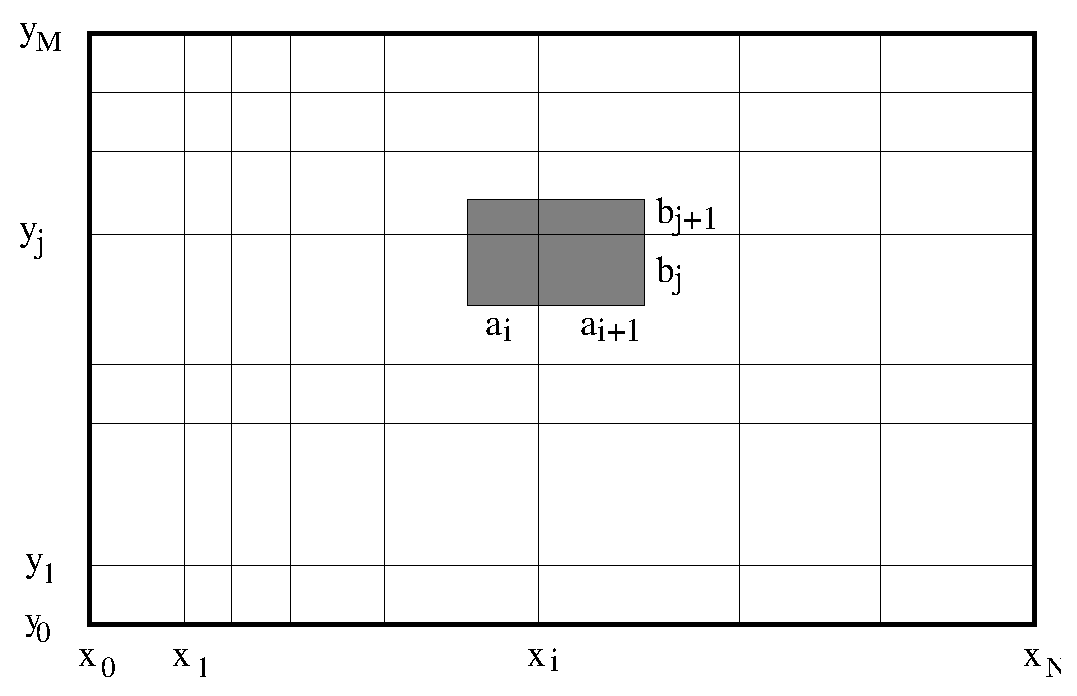
\includegraphics[width=2in] {bmgrid.eps} }
\caption{Discretization grid on the 2D domain $D$.  The box $C_{ij}$ of area
$s_{ij}=\frac{a_i+a_{i+1}}{2} \frac{b_i+b_{i+1}}{2}$ is shaded.}
\label{fig:bimgrid}
\end{figure}

We will have $N \times M$ internal nodes in which the function $\psi$ is unknown.
The function $\psi(x, y, t)$ in the points where $x = x_0$ or $x = x_{N+1}$ or $y = y_0$ or $y = y_{M+1}$
is known thanks to the Dirichlet boundary contitions.

In order to solve the TDSE we use here a vertex-centered Box Integration Method.
First, we consider the internal grid points and partially cover the domain $D$
with $N \times M$ boxes 
\begin{equation}
C_{ij} = [\frac{x_i - x_{i-1}}{2}, \frac{y_j - y_{j-1}}{2}] \times
                [\frac{x_{i+1} - x_i}{2}, \frac{y_{j+1} - y_j}{2}] ,
\end{equation}
where $i = 1, \cdots, N$ and $j = 1, \cdots, M$.

If we call $a_i = x_i - x_{i-1}$ and
$b_j = y_j - y_{j-1}$, the area of the box $C_{ij}$ is
$s_{ij} = \frac{a_i+a_{i+1}}{2} \frac{b_i+b_{i+1}}{2}$.
Following the Box Integration Method we integrate Eq.~(\ref{tdsenoconst}) on each box $C_{ij}$:
\begin{equation}
\int_{C_{ij}} \frac{\partial \psi}{\partial t} \, ds = 
   \beta \int_{C_{ij}} \nabla G \, ds + 
   \int_{C_{ij}} v \, \psi \, ds \, .
\end{equation}

The three integrals can be approximated as follow:
\begin{eqnarray}
\int_{C_{ij}} \frac{\partial \psi}{\partial t} \, ds & \approx &
   s_{ij} \frac{d \psi}{dt}(x_i, y_j, t) \, , \\
\int_{C_{ij}} v \, \psi \, ds & \approx & s_{ij} (v \psi)(x_i, y_j, t) \, , \\
\int_{C_{ij}} \nabla G \, ds = \oint_{\partial C_{ij}} G \bar{\ve{n}} \, dl & \approx &
   (G_e \bar{\ve n}_e + G_n \bar{\ve n}_n + G_w \bar{\ve n}_w + G_s \bar{\ve n}_s) \, ,
   \label{green_int}
\end{eqnarray}
where the Green's theorem has been used in the latter expression.
$\bar{\ve n}_e$, $\bar{\ve n}_n$, $\bar{\ve n}_w$ and $\bar{\ve n}_s$ are the vectors normal to the four
edges of the box ${C_{ij}}$, and whose modulus is equal to the lenght of the edge (area of the surface in the 3D case);
$G_e$, $G_n$, $G_w$ and $G_s$ are the values of $G$, namely the gradient of $\psi$, in the mid point of each edge, as shown in Fig~\ref{fig:single_box}.

\begin{figure}
\centerline{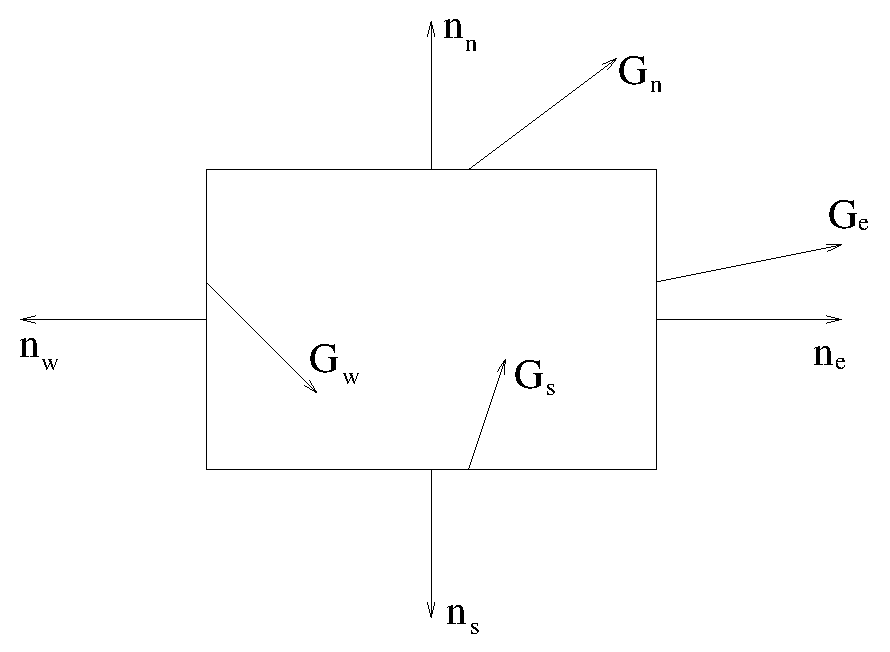
\includegraphics[width=2in] {box.eps} }
\caption{Single box scheme}
\label{fig:single_box}
\end{figure}

Let define the space-discretized wave function $\psi_{i,j}(t) = \psi(x_i, y_i, t)$.
For ease of notation, here we use a two-index representation for $\psi_{ij}$ although this quantity is
represented in the code as a 1D array.  Specifically, $\psi_{i,j}$ means that we are referring to the element ${iM+j}$.
Using a centered difference formula, the gradient values $G$ can be aproximated from the $\psi_{i,j}$ values on the nodes: 
\begin{eqnarray}
G_e \bar{\ve n}_e & \approx & \frac{\psi_{i,j}-\psi_{i-1,j}}{a_i} \frac{b_j+b_{j+1}}{2} \, ,      \\ \nonumber
G_n \bar{\ve n}_n & \approx & \frac{\psi_{i,j}-\psi_{i+1,j}}{a_{i+1}} \frac{b_j+b_{j+1}}{2} \, ,  \\ \nonumber
G_w \bar{\ve n}_w & \approx & \frac{\psi_{i,j}-\psi_{i,j-1}}{b_j} \frac{a_i+a_{i+1}}{2} \, ,      \\ \nonumber
G_s \bar{\ve n}_s & \approx & \frac{\psi_{i,j}-\psi_{i,j+1}}{b_{j+1}} \frac{a_i+a_{i+1}}{2} \, .     \nonumber
\end{eqnarray}

Let us now define
\begin{eqnarray}
k_1 &=& \frac{b_j+b_{j+1}}{2a_i}, \qquad k_2 = \frac{b_j+b_{j+1}}{2a_{i+1}}  \, ,      \\ \nonumber
k_3 &=& \frac{a_i+a_{i+1}}{2b_j}, \qquad k_4 = \frac{a_i+a_{i+1}}{2b_{j+1}}  \, .     \nonumber
\end{eqnarray}

The approximation of the integral in Eq.~(\ref{green_int}) becomes
\begin{eqnarray}
\lefteqn{\int_{C_{ij}} \nabla G \, ds \approx}   \\ \nonumber
& \approx &   (k_1+k_2+k_3+k_4) \, \psi_{i, j} + 
k_1 \, \psi_{i-1,j} + k_2 \, \psi_{i+1,j} + k_3 \, \psi_{i,j-1} + k_4 \, \psi_{i,j+1} \, .
\end{eqnarray}

If a box is adjacent to the boundary of the domain, some of the $\psi_{i,j}$ terms of the summation are defined by the boundary conditions rather than being unknown.  In this case we can group all these terms in one constant term.
For example, if $(i, j) = (1, 1)$, then $\psi_{i-1,j}$ and $\psi_{i,j-1}$ are on the boundaries and the above expression becomes
\begin{eqnarray}
\lefteqn{\int_{C_{11}} \nabla G \, ds \approx}   \\ \nonumber
& \approx &   (k_1+k_2+k_3+k_4) \, \psi_{1,1} + 
k_2 \, \psi_{2,1} + k_4 \, \psi_{1,2} + d_{11} \, .
\end{eqnarray}
where $d_{11} = k_1 \, \psi_{0,1} + k_3 \, \psi_{1,0}$ is the contant term that includes the known
values of $\psi$ at the boundaries.

In vector form, for each given box $C_{ij}$ these summations can be represented as a scalar product:
\begin{equation}
\ve m_{ij} \ve \psi + d_{ij} = \sum_{(k,l)=(1,1)}^{(N,M)} m_{ij}^{k,l} \, \psi_{k,l} + d_{ij}
\end{equation}
with $\ve \psi$ representing the column vector of the wave function and
with $\ve m_{ij} \in R^{N \times M}$ defined by
\begin{eqnarray}
\lefteqn{ \ve m_{ij} = (m_{ij}^{1,1}, m_{ij}^{1,2},\cdots, m_{ij}^{N,M}) = }  \\ \nonumber
&=&(0,\cdots, 0, \, k_1, 0, \cdots, 0, \, k_3, k_1+k_2+k_3+k_4, k_4 \, , 0,\cdots, 0, \, k_2, 0, \cdots, 0) \, .
\end{eqnarray}
Thus, the Schr\"{o}dinger equation can be approximately integrated on the box $C_{ij}$ with
\begin{equation}
s_{ij} \frac{d \psi_{i,j}}{dt}(t) = 
\beta \ve m_{ij} \ve \psi(t) + s_{ij} \, v_{ij} \, \psi_{i,j}(t) + \beta d_{ij} \, ,
\end{equation}
where $v_{ij}=v(x_i,x_j)$. 

By defining the diagonal matrices $S = \mbox{diag}(s_{ij})$ and $V = \mbox{diag}(v_{ij})$,
and the matrix whose columns are the vectors $\ve m_{ij}$: $M = \beta [\ve m_{ij}]$,
the equation can be written in matrix form:
\begin{equation} \label{tdsematrixform}
S \frac{d \ve \psi}{dt}(t) = M \ve \psi(t) + S V \ve \psi + \beta \ve d \, ,
\end{equation}
where the vector symbol $\ve d$ represents the column vector
$\ve d = (d_{11}, d_{12},\cdots, d_{NM})$, as usual.

For the \emph{time discretization} we use a Cranck-Nicholson scheme (also known as
trapezoidal rule).  By considering a time step $\Delta_t$, Eq.~(\ref{tdsematrixform}) becomes:
\begin{equation}
S {\ve \psi}(t+\Delta_t) = S \ve \psi(t) + \frac{(M+SV)\Delta_t}{2} 
\left( \ve \psi(t) + \ve \psi(t+\Delta_t) \right) + \beta \Delta_t \ve d
\end{equation}
or equivalently
\begin{equation} \label{CNmatrix}
\left( S - \frac{(M+SV)\Delta_t}{2} \right) \ve \psi(t+\Delta_t) =
\left( S + \frac{(M+SV)\Delta_t}{2} \right) \ve \psi(t) + \beta \Delta_t \ve d
\end{equation}

Note that in case the potential $v$ is dependent on the time, the two matrices $V$ on
the left and right sides of Eq.~(\ref{CNmatrix}) must be computed at the later and earlyer
time step, respectively.
By making explicit the above equation for $\psi(t+\Delta_t)$ one gets
\begin{equation}
\ve \psi(t+\Delta_t) =
\frac{ 2\beta \Delta_t \ve d \ + \ \left(2S + \left( M+S\,V(t) \right)\Delta_t\right) \ve \psi(t) }
{2S - \left( M+S\,V(t+\Delta_t)\right)\Delta_t}
\end{equation}

\section{Nonlinear Scr\"{o}dinger equation}
The time-dependent nonlinear Shroedinger equation can be stated as follow:

$$ i \hbar \frac{\partial}{\partial t} \psi =
   -\frac{\hbar^2}{2m^*} \bigtriangledown^2 \psi +
   \left(V(x) + \frac{4 \pi \hbar^2 a_s}{m^*} |\psi|^2 \right) \psi $$

In this case we suppose a periodic boundary condition. We can rewrite the equation by highliting the linear part and the nonlinear part of the operator:

\begin{eqnarray}
\frac{\partial}{\partial t} \psi & = & L \psi + N \psi \label{eq:splitop} \\
\psi(x, 0) & = & \psi_0(x)
\end{eqnarray}

with
$$ L = \frac{i\hbar}{2m^*} \bigtriangledown^2 \ , \qquad
   N = -i \left(\frac{1}{\hbar}V(x) + \frac{4 \pi \hbar a_s}{m^*} |\psi|^2 \right) $$

\section{Split-step Fourier Method}
Split-step method can be effectively used to solve time dependent problems in the form of \ref{eq:splitop}.
In particular, the solution of Equation \ref{eq:splitop} may be advanced from one time level to the next by means of the following formula:

$$ \psi(x, t+dt) = e^{dt(L+N)} \psi(x, t) \label{eq:split1} $$

where $dt$ denotes the time step. In general, Equation \ref{eq:split1} is first order accurate; however it becomes exact if the operators $L$ and $N$ are time-independent (\ref{bib:SIAM}).
The analytic expression of $e^{dt(L+N)}$ is usually not known, as in the case of the nonlinear Schroedinger equation. However we can show some expressions for approximating it with different order of accuracy.

First order approximation:
$$ A_1(dt) = e^{dtL} e^{dtN} \label{eq:split2} $$

Second order approximation:
$$ A_2(dt) = e^{\frac{1}{2}dtN} e^{dtL} e^{\frac{1}{2}dtN} $$

Fourth order approximation:
$$ A_4(dt) = A_2(wdt) A_2((1-2w)dt) A_2(wdt) \, \quad
   w = \frac{2+\sqrt[3]{2} + \frac{1}{\sqrt[3]{2}}}{3} $$

As an esample, we see that the equation $ \psi_t = A_1(dt) \psi $
is equivalent to first solve the nonlinear equation $ \psi_t = N \psi $
and then advancing the solution by solving the linear equation $ \psi_t = L \psi $.

In the case of the nonlinear Schroedinger equation, the nonlinear step $ \psi_t = N \psi $ can be computed with:
$$ \psi_n(x_i, t) = \psi(x_i, t) e^{-i dt \left(\frac{1}{\hbar}V(x_i) + \frac{4 \pi \hbar a_s}{m^*} |\psi(x_i, t)|^2 \right)} $$

For the linear step $ \psi_t = L \psi $, the analytical solution is known and it can be computed in the $k$ space by means of a Fourier transform.

\begin{eqnarray}
 \bar{\psi}(t) &=& \mbox{FFT}(\psi(t)) \\
 \bar{\psi}(k_i, t+dt) &=& \bar{\psi}(k_i, t) e^{dt \frac{i\hbar}{2m^*} k_i^2} \label{eq:klinearevolution} \\
 \psi(t+dt) &=& \mbox{IFFT}(\bar{\psi}(t+dt))
\end{eqnarray}

In case of a 2D wave function, the linear transformation of Equation \ref{eq:klinearevolution} becomes
$$ \bar{\psi}(k_i, k_j, t+dt) = \bar{\psi}(k_i, t)
   e^{dt \frac{i\hbar}{2m^*} (k_i^2 + k_j^2)} \label{eq:klinearevolution} $$

It is important to properly define the frequency components $k_i$.
In particular, if the wave function is defined on $[0, s]$ it is discrtized on $n$ points, then the $k_i$ are defined as:

\begin{equation} k_i = \left\{ \begin{array}{rll}
          &\frac{2 \pi (i-1)}{s} & i = 1, \ldots, \frac{n}{2} \\
          -&\frac{2 \pi (n-i+1)}{s} & i = \frac{n}{2}+1, \ldots, n \\
         \end{array} \right . \end{equation}

\newpage

\begin{appendices}
\section{Notation}

The following notation will be used for the spatial derivatives of a complex functional
$f:(x_1,\cdots, x_n)\mapsto C$:
\begin{eqnarray}
\nabla f &=& \mbox{grad}(f) =
\left( \frac{\partial f}{\partial x_1}, \cdots, \frac{\partial f}{\partial x_n} \right) \\
\nabla \cdot f &=& div(f) = \frac{\partial f}{\partial x_1} + \cdots + \frac{\partial f}{\partial x_n} \\
\nabla^2 f &=& \nabla \cdot \nabla f =
    \frac{\partial^2 f}{\partial x_1^2} + \cdots + \frac{\partial^2 f}{\partial x_n^2}
\end{eqnarray}

\end{appendices}

\begin{thebibliography}{2}
\bibitem{bib:SIAM}
Weideman, J.A.C., Herbst B.M.: Split-step methods fo the solution of the nonlinear Schroedinger equation, SIAM J. Numer. Anal. \textbf{23}(3), 485-507, (1986)

\bibitem{bib:parsplitstep}
Xu X., Taha T., Parallel split-step fourier methods for nonlinear schroedinger-type equations, J. Math Model. Algo. \textbf{2}, 185-201, (2003)

\end{thebibliography}

\end{document}
